\documentclass[10pt,a4paper,titlepage]{report}
\usepackage[utf8]{inputenc}
\usepackage{amsmath}
\usepackage{amsfonts}
\usepackage{amssymb}
\usepackage{graphicx}
\usepackage{xcolor}
\usepackage{minted}

\newcommand{\HRule}[1]{\rule{\linewidth}{#1}}

\nonstopmode


\begin{document}
{\fontfamily{cmr}\selectfont
\title{ \normalsize \textsc{}
\\ [2.0cm]
\HRule{0.5pt} \\
\LARGE \textbf{\uppercase{Cursors}
\HRule{2pt} \\ [0.5cm]
\normalsize \today \vspace*{5\baselineskip}}
}

\date{}

\author{
	Rwithik Manoj \\
	College of Engineering, Trivandrum \\
	Department of Computer Science and Engineering }

\maketitle
\newpage

\sectionfont{\scshape}

\begin{enumerate}
		\item Create table student (id, name, m1, m2, m3, grade). Insert 5 tuples into it. Find the total, calculate grade and update the grade in the table.
	\begin{verbatim}

CREATE OR REPLACE FUNCTION grader()
RETURNS INTEGER
AS $$
DECLARE
	cur CURSOR FOR SELECT * FROM student;
	rec RECORD;
	total INTEGER;
	grd CHAR(1);
BEGIN
	OPEN cur;
	LOOP
		total := 0;
		FETCH cur into rec;
		EXIT WHEN NOT FOUND;
		total := rec.m1 + rec.m2 + rec.m3;
		IF total > 250 THEN
			grd := 'A';
		ELSIF total > 200 THEN
			grd := 'B';
		ELSIF total > 150 THEN
			grd := 'C';
		ELSIF total > 100 THEN
			grd := 'D';
		ELSE
			grd := 'F';
		END IF;
		UPDATE student SET grade = grd WHERE CURRENT OF cur;
	END LOOP;
	CLOSE cur;
	RETURN null;
END;
$$ LANGUAGE plpgsql;
	\end{verbatim}
	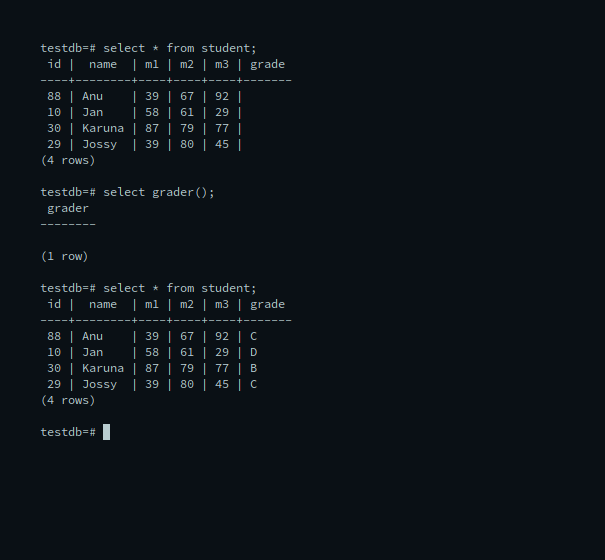
\includegraphics[width=\linewidth]{../Images/Cursors/1.png}

	\item Create bank\_details (accno, name, balance, adate).Calculate the interest of the amount and insert into a new table with fields (accno, interest). Interest = 0.08 * balance.\newline
	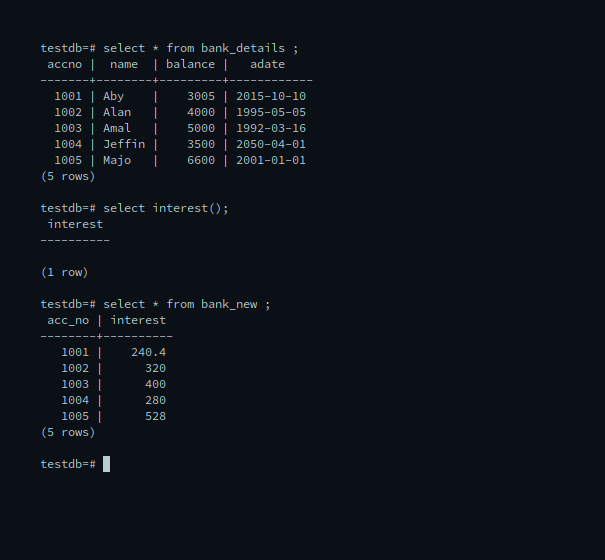
\includegraphics[width=\linewidth]{../Images/Cursors/2.png}
	\begin{verbatim}
	
CREATE OR REPLACE FUNCTION interest()
RETURNS INTEGER
AS $$
DECLARE
	cur CURSOR FOR SELECT * FROM bank_details;
	rec RECORD;
	intr REAL;
BEGIN
	CREATE TABLE bank_new(acc_no int, interest real);
	OPEN cur;
	LOOP
		FETCH cur into rec;
		EXIT WHEN NOT FOUND;
		intr := rec.balance * 0.08;
		INSERT INTO bank_new VALUES(rec.accno, intr);
	END LOOP;
	CLOSE cur;
	RETURN null;
END;
$$ LANGUAGE plpgsql;
	\end{verbatim}

	\item Create table people\_list (id, name, dt\_joining, place).If person’s experience is above 10 years, put the tuple in table exp\_list (id, name, experience).\newline
	\begin{verbatim}

CREATE OR REPLACE FUNCTION exp()
RETURNS INTEGER
AS $$
DECLARE
	cur CURSOR FOR SELECT * FROM people_list;
	rec RECORD;
BEGIN
	OPEN cur;
	LOOP
		FETCH cur into rec;
		EXIT WHEN NOT FOUND;
		IF rec.dt_joining < '2009-08-18' THEN
			INSERT INTO exp_list VALUES(rec.id, rec.name, ('2019-08-18' - rec.dt_joining)/365);
		END IF;
	END LOOP;
	CLOSE cur;
	RETURN null;
END;
$$ LANGUAGE plpgsql;
	\end{verbatim}
	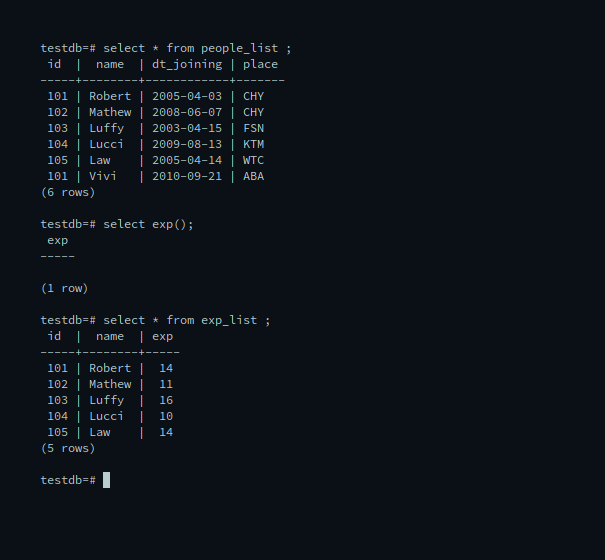
\includegraphics[width=\linewidth]{../Images/Cursors/3.png}
\item Create table
employee\_list(id,name,monthly salary). If:\newline
  annual salary less than 60000, increment monthly salary by 25\% \newline
  between 60000 and 200000, increment by 20\%\newline
  between 200000 and 500000, increment by 15\%\newline
  annual salary greater than 500000, increment monthly salary by 10\%\newline
	\begin{verbatim}

CREATE OR REPLACE FUNCTION sal()
RETURNS INTEGER
AS $$
DECLARE
	cur CURSOR FOR SELECT * FROM employee_list;
	rec RECORD;
BEGIN
	OPEN cur;
	LOOP
		FETCH cur into rec;
		EXIT WHEN NOT FOUND;
		IF (rec.salary * 12) < 60000 THEN
			UPDATE employee_list SET salary = salary * 1.25 WHERE CURRENT OF cur;
		ELSIF (rec.salary * 12) < 200000 THEN
			UPDATE employee_list SET salary = salary * 1.2 WHERE CURRENT OF cur;
		ELSIF (rec.salary * 12) < 500000 THEN
			UPDATE employee_list SET salary = salary * 1.15 WHERE CURRENT OF cur;
		ELSE
			UPDATE employee_list SET salary = salary * 1.1 WHERE CURRENT OF cur;
		END IF;
	END LOOP;
	CLOSE cur;
	RETURN null;
END;
$$ LANGUAGE plpgsql;
	\end{verbatim}
	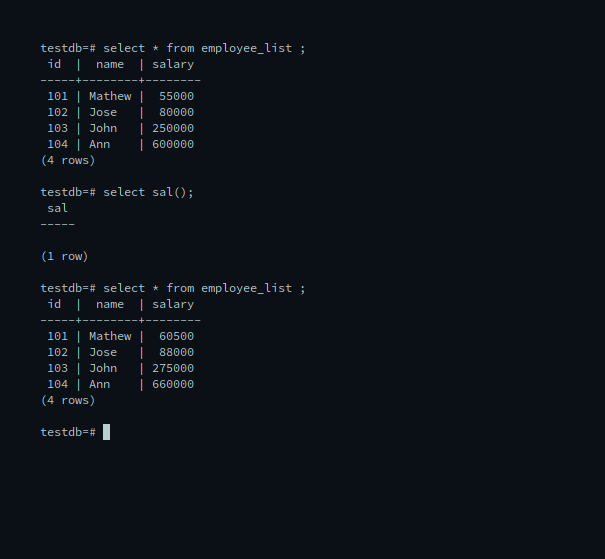
\includegraphics[width=\linewidth]{../Images/Cursors/4.png}

\end{enumerate}

\subsubsection{RESULT}
The PL/SQL programs were executed successfully and the output was obtained.

}
\end{document}
